\documentclass{article}
\usepackage{amsmath}
\usepackage{amssymb}
\usepackage{amsfonts}
\usepackage{braket}
\usepackage{hyperref}
\usepackage{graphicx}
\usepackage{caption}
\usepackage{geometry}
\geometry{a4paper, margin=1in}
\newcommand{\source}[1]{\caption*{Source: {#1}} }
\captionsetup[figure]{font=small,labelfont= small}
\title{The Quantum Conundrum: Redefining Security in the Quantum Revolution}
\author{Shibraj S.}
\date{January 2025}

\begin{document}

\maketitle

\section*{Introduction}

In the age of digital communication, encryption is crucial for ensuring the privacy and security of data exchanged over the internet. The advent of quantum computing represents a paradigm shift in computational capabilities, bringing both remarkable opportunities and profound challenges. Among the most affected fields is cryptography, the cornerstone of secure digital communication. This article explores both sides of quantum computing's impact on cryptography, focusing on the vulnerabilities it introduces to classical encryption schemes and the secure possibilities offered by protocols like Quantum Key Distribution (QKD).

\section*{Shor's Algorithm and the Threat to Classical Cryptography}

At the heart of modern cryptography lie hard mathematical problems, such as integer factorization (used in RSA encryption) and discrete logarithms (used in Elliptic Curve Cryptography, or ECC). These problems are computationally infeasible for classical computers to solve within a reasonable timeframe, providing the security guarantees we rely on for digital communication.

Enter quantum computing, which disrupts this status quo. In 1994, Peter Shor introduced a quantum algorithm capable of efficiently solving these problems. The subsequent section will outline how this algorithm works in the case of RSA encryption.
\begin{figure}[h]
    \centering
    \includegraphics[width = 7.00cm\textwidth]{shor.jpg}
     \caption*{Peter Shor (b. 1959)}
\end{figure}

RSA encryption, named after its creators, Rivest, Shamir, and Adleman, is one of the most widely used public-key cryptosystems. It relies on the difficulty of factoring large composite numbers that are the product of two large prime numbers. Given below is an overview of how the keys are generated in RSA encryption.

\paragraph{Key Generation in RSA:}
\begin{enumerate}
    \item  First, choosing two sufficiently large prime numbers, $p$ and $q$.
    \item  Computing $N = p \times q$ .
    \item Calculating $\phi(N) = (p-1)(q-1)$, the *totient of $N$.
    \item Selecting a public exponent $e$ such that $1 < e < \phi(N)$ and $\gcd(e, \phi(N)) = 1$.
    \item Computing the private key $d$ as the modular multiplicative inverse of $e \mod \phi(N)$, satisfying $e \cdot d \equiv 1 \mod \phi(N)$.
\end{enumerate}

* (The totient of N counts all integers upto N that do not share any prime factors with N) \\

\begin{figure}[h]
    \centering
    \includegraphics[width = 10.00cm\textwidth]{rsa.png}
     \caption{RSA Encryption}
    \source{\href{https://github.com/AbdullahAlhussein/RSA-Algorithm}{Github}}
   
\end{figure}

RSA encryption allows anyone to encrypt a message using the recipient's public key \((N, e)\). The ciphertext \(c\) is computed as \(c = m^e \mod N\), where \(m\) is the message. Decrypting the ciphertext requires the private key \(d\), which is computationally infeasible to derive without factoring \(N\), ensuring security. For sufficiently large $N$ (e.g., 2048 bits), classical algorithms cannot factorize $N$ within a practical timeframe. To give a rough estimate, one of the best-known classical algorithms for integer factorization, the General Number Field Sieve (GNFS), with a sub-exponential time complexity (faster than polynomial time but slower than exponential) could factor a 795-bit number in about two years using huge computational resources.
This gives a rough idea of the arduous task classical decryption has to face.
\subsection*{How Shor’s Algorithm Breaks RSA ?}

Shor’s algorithm revolutionizes the factoring problem by providing an efficient quantum solution. It consists of two main steps:

\paragraph{Reduction to Period Finding:}
\begin{itemize}
    \item Given $N = p \times q$ and a random integer $a$ such that $1 < a < N$, define the function:
    \begin{equation*}
        f(x) = a^x \mod N.
    \end{equation*}
    \item The function $f(x)$ is periodic with a period $r$. Shor’s algorithm exploits this periodicity to factor $N$.
\end{itemize}

\paragraph{Quantum Period Finding:}
\begin{itemize}
    \item The quantum computer constructs a superposition of states (this will be discussed later) and applies the Quantum Fourier Transform (quantum analog of the classical discrete Fourier transform) to determine the period $r$.
    \item Once $r$ is found, classical post-processing is used to compute the factors of $N$. Specifically, if $r$ is even, then:
    \begin{equation*}
        \gcd\left(a^{r/2} - 1, N\right) \quad \text{and} \quad \gcd\left(a^{r/2} + 1, N\right)
    \end{equation*}
    yield the factors of $N$.
\end{itemize}

\subsection*{Why Shor’s Algorithm is a Game-Changer ?}

As already mentioned, the best classical algorithms for factoring, such as the General Number Field Sieve, have a sub-exponential time complexity. In contrast, Shor’s algorithm has a polynomial time complexity of $O((\log N)^3)$, making it exponentially faster. This efficiency renders RSA insecure against quantum computers capable of running Shor’s algorithm.

For example, a 2048-bit RSA key, which is currently considered secure, can be broken in polynomial time with Shor’s algorithm once a sufficiently powerful quantum computer is built (one using more than 10 million logical qubits). Though the present day scenario of quantum computing with at most hundreds of noisy qubits do not pose an immediate threat,  this imminent vulnerability underscores the urgency of transitioning to quantum-resistant cryptographic systems.




\section*{From Breaking Encryption to Securing It}
While quantum computing threatens traditional cryptography, it also provides tools for securing communication. Quantum Key Distribution (QKD) is a prime example, offering provably secure key exchange based on quantum mechanics.
Before diving into QKD, let us define key quantum terms that will help us understand QKD.

\subsubsection*{Quantum State and Superposition}

In quantum mechanics, the state of a quantum system is described by a \textit{state vector}, or \textit{ket}, denoted by \( |\psi\rangle \). For a qubit, the state vector is a linear combination of the basis states \( |0\rangle \) and \( |1\rangle \), known as the computational basis:
\[
|\psi\rangle = \alpha |0\rangle + \beta |1\rangle,
\]
where \( \alpha, \beta \in \mathbb{C} \) (Field of Complex numbers), and the normalization condition
\[
|\alpha|^2 + |\beta|^2 = 1
\]
ensures that the total probability of measuring the qubit in one of its basis states is 1.

The coefficients \( \alpha \) and \( \beta \) represent the probability amplitudes of measuring the qubit in the states \( |0\rangle \) and \( |1\rangle \), respectively. The probabilities of measuring \( |0\rangle \) and \( |1\rangle \) are given by \( |\alpha|^2 \) and \( |\beta|^2 \), respectively.
This phenomenon of a qubit being in a superposition of both \( |0\rangle \) and \( |1\rangle \) until measured is known as quantum \textit{superposition}.
\begin{figure}[h]
    \centering
    \includegraphics[width = 9.00cm\textwidth]{qubit_processed.jpg}
     \caption{Bloch Sphere representing a Qubit}
   
\end{figure}
\subsubsection*{Quantum Entanglement}

\textit{Quantum entanglement} refers to the phenomenon where two or more quantum particles become "linked", such that the state of one particle is immediately correlated with the state of the other(s). If two qubits are entangled, measuring one qubit instantly provides information about the state of the other.

Consider an entangled state, commonly known as a Bell state:
\[
|\Phi^+\rangle = \frac{1}{\sqrt{2}} \left( |00\rangle + |11\rangle \right).
\]
If one qubit in the pair is measured to be \( |0\rangle \), the other will necessarily be in the state \( |0\rangle \), and similarly for \( |1\rangle \). This apparent "non-locality" by no means hints at faster-than-light information transfer, which is still a local phenomenon. 

\subsubsection*{Quantum Measurement}

The act of \textit{measurement} in quantum mechanics collapses the quantum state into one of its eigenstates, with the probability of each outcome determined by the square of the coefficient of the corresponding eigenstate. If a qubit is in a superposition \( |\psi\rangle = \alpha |0\rangle + \beta |1\rangle \), a measurement of the qubit will yield \( |0\rangle \) with probability \( |\alpha|^2 \) and \( |1\rangle \) with probability \( |\beta|^2 \).


\section*{Quantum Key Distribution (QKD)}

Quantum Key Distribution (QKD) involves transmitting information using quantum states, to ensure that any eavesdropping is immediately detectable.  QKD utilizes the principles of quantum mechanics to allow two parties to securely exchange cryptographic keys. The most well-known QKD protocol is the \textit{BB84 protocol}, developed by Charles Bennett and Gilles Brassard in 1984. 

Let Alice and Bob be the two individuals who wish to securely share a secret key over an insecure channel with BB84 protocol. The protocol is based on the idea that quantum measurement disturbs quantum states, and this disturbance can be detected. Let us now examine how Alice can securely transmit information to Bob with this protocol.
\subsubsection*{Step 1}

Alice prepares a sequence of \( n \) qubits, each randomly chosen from one of the two bases:
\begin{itemize}
    \item \textbf{Computational Basis:} \( |0\rangle, |1\rangle \),
    \item \textbf{Diagonal Basis:} \( |+\rangle = \frac{1}{\sqrt{2}}(|0\rangle + |1\rangle), \; |-\rangle = \frac{1}{\sqrt{2}}(|0\rangle - |1\rangle). \)
\end{itemize}
Each qubit encodes a classical bit \( b \in \{0, 1\} \), with the following mappings:
\[
b = 0 \implies |0\rangle \text{ or } |+\rangle, \quad b = 1 \implies |1\rangle \text{ or } |-\rangle.
\]
Alice records both the bit value \( b \) and the chosen basis for each qubit.

\subsubsection*{Step 2}

Alice sends the sequence of \( n \) qubits to Bob over a quantum channel. The qubits are transmitted in the chosen basis, but the basis itself is not revealed to Bob.

\subsubsection*{Step 3}

Bob measures each received qubit in a randomly chosen basis (computational or diagonal). If Bob's measurement basis matches Alice's preparation basis, the measurement outcome will correctly match Alice's encoded bit. Otherwise, the outcome is random due to the incompatibility of the bases.

\subsubsection*{Step 4}

After the transmission and measurement steps, Alice and Bob publicly announce the bases they used for each qubit (but not the actual measurement outcomes or encoded bits). They discard all qubits where their bases do not match. The remaining qubits form the shared raw key.

\subsubsection*{Eavesdropping Detection}
If an eavesdropper, Eve, intercepts the qubits, she will be forced to measure the qubits in a random basis. Due to the principles of quantum measurement, Eve’s measurements will disturb the quantum states, introducing errors into the transmitted key. 
\begin{figure}[h]
    \centering
    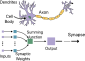
\includegraphics[width = 7.00cm\textwidth]{fig1.png}
     \caption{QKD Model}
    \source{\href{https://www.cse.wustl.edu/~jain/cse571-07/ftp/quantum/}{Washinton Uni. article}}
   
\end{figure}

To detect eavesdropping, Alice and Bob compare a randomly selected portion of the raw key. If the error rate exceeds a predefined threshold \( \epsilon \), they abort the protocol, assuming that an eavesdropper (Eve) was present.


\section*{Security of QKD}

The security of QKD relies on two of these important quantum principles:

\subsubsection*{No-Cloning Theorem}

The \textit{no-cloning theorem} states that it is impossible to create an identical copy of an unknown quantum state. This ensures that any attempt to intercept the qubits and measure them will necessarily disturb the quantum state, revealing the presence of the eavesdropper.

\subsubsection*{Heisenberg Uncertainty Principle}

The Heisenberg uncertainty principle asserts that certain pairs of physical quantities, such as position and momentum, cannot be precisely measured simultaneously. For QKD, this principle ensures that any attempt by Eve to measure the quantum states of the qubits will cause uncertainty and thus, an error in the measurement, thereby disturbing the qubits and alerting Alice and Bob to the eavesdropping.

\section*{Balancing Risks and Rewards}
The rise of quantum computing necessitates a paradigm shift in cryptography. While algorithms like Shor’s threaten traditional cryptographic systems, QKD protocols like BB84 exemplify the potential of quantum mechanics to safeguard communication. The developments in quantum computing challenges us to innovate, ensuring that the promise of this technology is harnessed securely and responsibly.

As we stand on the brink of the second quantum revolution, the interplay between threat and solution in cryptography is a testament to the dual nature of technological progress - both a challenge and an opportunity.

\section*{References}
\begin{enumerate}
    \item Shor, P. W. (1994). Algorithms for quantum computation: Discrete logarithms and factoring. Proceedings of the 35th Annual Symposium on Foundations of Computer Science, 124–134. 
    
     \href{https://doi.org/10.1109/SFCS.1994.365700}{https://doi.org/10.1109/SFCS.1994.365700}
    \item Gisin, N., Ribordy, G., Tittel, W., \& Zbinden, H. (2002). Quantum cryptography. Reviews of Modern Physics, 74(1), 145–195. 
    
     \href{https://doi.org/10.1103/RevModPhys.74.145}{https://doi.org/10.1103/RevModPhys.74.145}
    \item Mehic, M., Niemiec, M., Rass, S., Ma, J., Peev, M., Aguado, A., Martin, V., Schauer, S., Poppe, A., Pacher, C., \& Voznak, M. (2020). Quantum Key Distribution: A Networking Perspective. ACM Computing Surveys, 53(4), Article 71. 
    
     \href{https://dl.acm.org/doi/10.1145/3402192}{https://dl.acm.org/doi/10.1145/3402192}

     \item Gitonga, C. K. (2024). The Impact of Quantum Computing on Cryptographic Systems: Urgency of Quantum-Resistant Algorithms and Practical Applications in Cryptography. European Journal of Information Technologies and Computer Science (EJ-COMPUTE), 1(1), Article 146.
     \href{https://www.ej-compute.org/index.php/compute/article/view/146}{https://www.ej-compute.org/index.php/compute/article/view/146}

     \item Cobb, M. (2021). RSA Algorithm. $\textbf{TechTarget}$
     
     \href{https://www.techtarget.com/searchsecurity/definition/RSA}{https://www.techtarget.com/searchsecurity/definition/RSA}
    \item Beller, M. (2016). Quantum Mechanics from The Stanford Encyclopedia of Philosophy (E. N. Zalta, Ed.)
    
   \href{https://plato.stanford.edu/entries/qm/}{https://plato.stanford.edu/entries/qm/} 

\end{enumerate}
\end{document}
